\newpage
\hypertarget{t2m close}{}
\subsection{Tree To Model Close}
\genHeader

\begin{itemize}

\item[$\blacktriangleright$] Navigate to ``src/org.moflon.tie'' right click and run TGGMain as application.

\begin{figure}[htbp]
\begin{center}
  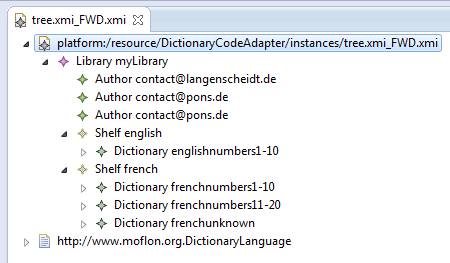
\includegraphics[width=0.7\textwidth]{eclipse_generatedForwardTransformation}
  \caption{completed forward transformation}
  \label{eclipse:generatedFwdTrsfm}
\end{center}
\end{figure}

\item[$\blacktriangleright$] Awesome, it works BEAUTIFULLY! Lets examine the output, \texttt{tree.xmi\_FWD.xmi} a little closer.

\item[$\blacktriangleright$] If you haven't already, read Section 6 from Part IV to learn how eMoflon's integrator feature can help you visualize how this
transformation was completed. Run the integrator on \texttt{corr\_FWD.xmi} until you reach the first (english) author node (do this as proof).

\begin{figure}[htbp]
\begin{center}
  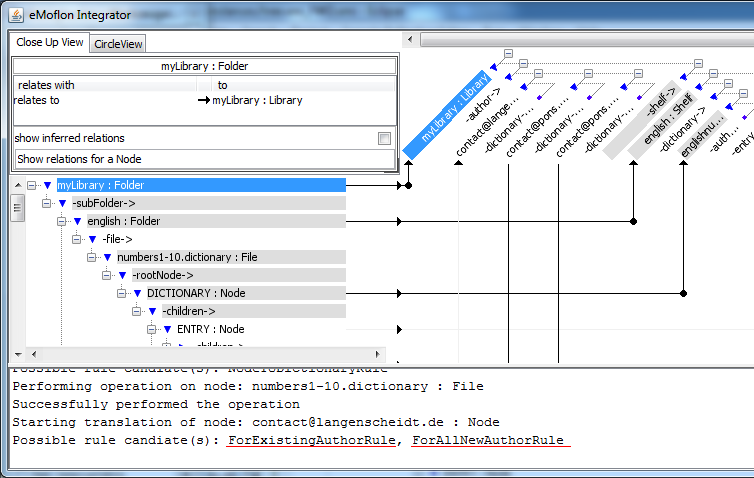
\includegraphics[width=0.7\textwidth]{eclipse_integratorAuthorChoice}
  \caption{completed forward transformation}
  \label{eclipse:generatedFwdTrsfm}
\end{center}
\end{figure}

\item[$\blacktriangleright$] The transformation decided to take one rule - either create or use existing - based on a random choice. The current set up isn't
dependable. We need to force a decision.

\item[$\blacktriangleright$] It had two choices and picked on at random. If you DO want to force a decision. You have two choices: ``I
don't care, \emph{always} make an author'' (duplicates), or no, ``I \emph{never} want there to be two of the same authors for one library.'' There are two ways
to define this: (Discuss options here?)

\end{itemize}

\begin{description}

\item[option1: Run-time] Create a configuration file for your TGG;

First: define \texttt{AuthorConfiguator}. FIG. put in in the same pacakage as your TGG. Don't make errors.

\begin{figure}[htbp]
\begin{center}
  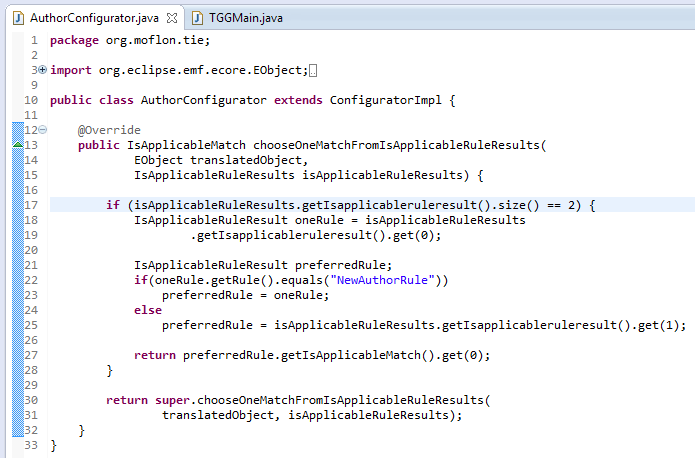
\includegraphics[width=0.7\textwidth]{eclipse_authorConfigurator}
  \caption{comment}
  \label{eclipse:authorConfig}
\end{center}
\end{figure}

Second: call it from \texttt{TGGMain}. FIG. Only need it in the forward transformation, so only put it once\ldots

\begin{figure}[htbp]
\begin{center}
  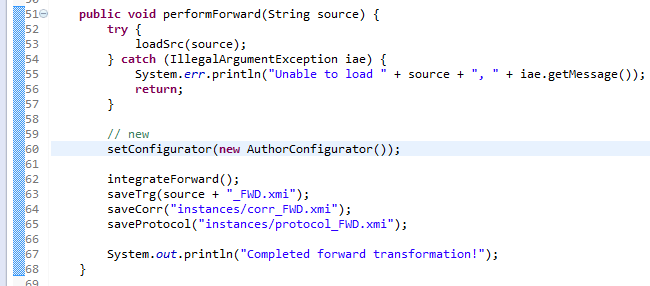
\includegraphics[width=0.7\textwidth]{eclipse_editTGGMain}
  \caption{comment on the edit}
  \label{eclipse:editTGGMain}
\end{center}
\end{figure}

\newpage

\item[option2: Design-time] Create a NAC in \texttt{ForAllNewAuthors}; force it to skip
\hyperlink{NAC vis}{link1: {\bf VISUAL}}
\hyperlink{NAC tex}{link2: {\bf TEXTUAL}}

\hypertarget{NAC vis}{}
\subsubsection{VISUAL NAC}
\texHeader

\begin{itemize}

\item[$\blacktriangleright$] Add the following to \texttt{NewAuthor}

\begin{figure}[htbp]
\begin{center}
  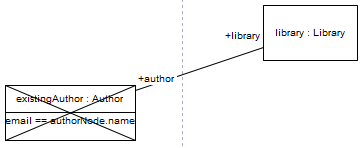
\includegraphics[width=0.7\textwidth]{ea_existingAuthorNAC}
  \caption{comment}
  \label{ea:existingAuthorNAC}
\end{center}
\end{figure}

\end{itemize}


\hypertarget{NAC tex}{}
\subsection{TEXTUAL NAC}
\texHeader

\begin{itemize}

\item[$\blacktriangleright$] Re-open \texttt{ForAllNewAuthor}. Add a NAC below \texttt{library} as depicted in FIG. If we had \emph{just} the library link,
then this rule would fail if the library had \emph{any} authors already set. So intead, we must add the email attribute constraint to match.

\begin{figure}[htbp]
\begin{center}
  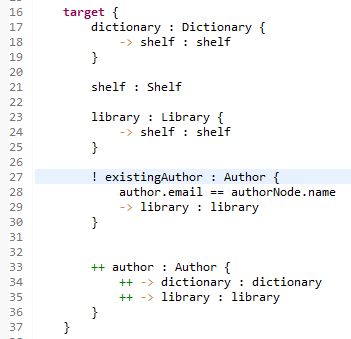
\includegraphics[width=0.7\textwidth]{eclipse_targetNAC}
  \caption{comment}
  \label{eclipse:existingAuthorNAC}
\end{center}
\end{figure}

\end{itemize}


\end{description}

% Back together, run TGGMain again
\newpage
\begin{itemize}

\item[$\blacktriangleright$] With your forced set up now constructed, Run TGGMain again. Use the integrator once more to see how it consistently chose your
decision.

\item[$\blacktriangleright$] Great work! You have now completed the first half of the complete round trip transformation, from Text to Model!

\end{itemize}
